\begin{fframe}
    \begin{block}
    {Beispiel: Fibonacci-Folge}
    \begin{align*}
        fib(1) &= fib(2) = 1 \\
        fib(n) &= fib(n-1) + fib(n-2)
    \end{align*}
    \end{block}
    \begin{block}<2->
    {die ersten 10 Fibonacci-Zahlen:}
    \begin{align*}
        \begin{array}{r|r|r|r|r|r|r|r|r|r|r}
            n: & 1 & 2 & 3 & 4 & 5 & 6 & 7 & 8 & 9 & 10\\
            \hline
            fib(n): & 1 & 1 & 2 & 3 & 5 & 8 & 13 & 21 & 34 & 55
        \end{array}
    \end{align*}
    \end{block}
\end{fframe}

\begin{fframe}
    \begin{block}
    {Beispiel: Hailstone-Folge}
    \begin{itemize}
        \item Beginne mit einer \emph{natürlichen Zahl} $n$.
        \item Ist $n$ gerade, so nimm als nächstes $n/2$.
        \item Ist $n$ ungerade, so nimm als nächstes $3n+1$.
        \item Wiederhole, bis der Zyklus $4,2,1$ erreicht ist.
    \end{itemize}
    \end{block}
    \begin{block}
    {Beispiele:}
    \begin{description}
        \item<2->[$n = 1$:] $1,4,2,1$
        \item<3->[$n = 2$:] $2,1,4,2,1$
        \item<4->[$n = 3$:] $3,10,5,16,8,4,2,1$
        \item<5->[$n = 4$:] $4,2,1$
        \item<6->[$n = 5$:] $5,16,8,4,2,1$
        \item<7->[$n = 6$:] $6,3,10,5,16,8,4,2,1$
        \item<8->[$n = 7$:] $7,22,11,34,17,52,26,13,40,20,10,5,16,8,4,2,1$
    \end{description}
    \end{block}
\end{fframe}

\begin{fframe}
    \begin{block}{Rekursion kann malen ...}
        \centering{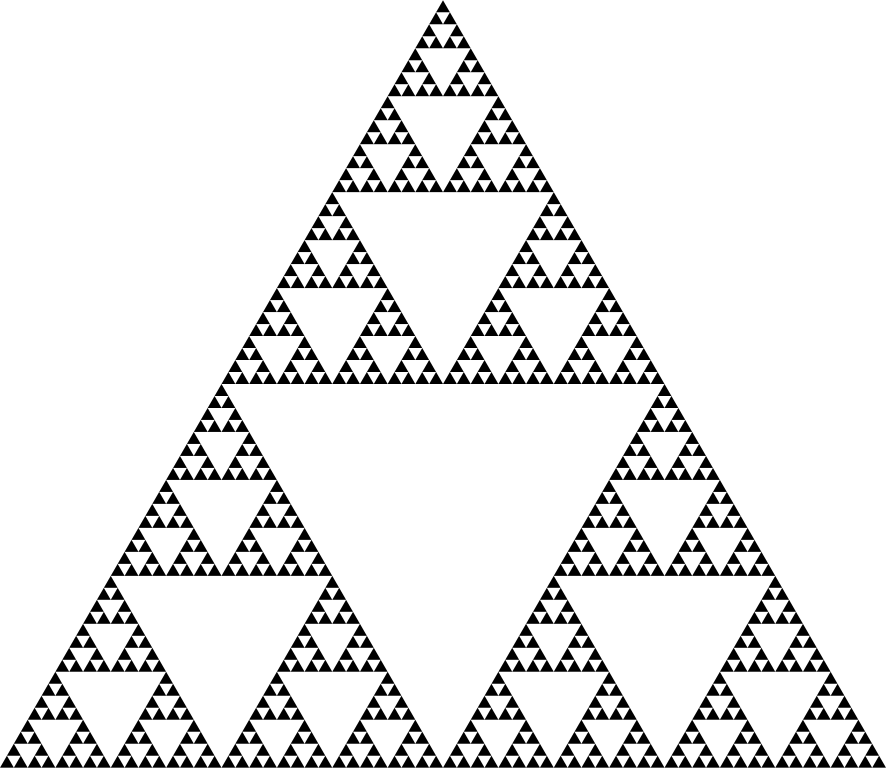
\includegraphics[scale=0.2]{sierpinski.png}}
    \end{block}
    \begin{block}{Dieses Bild wird \alert{Sierpinski-Dreieck} genannt.}
    \end{block}
\end{fframe}

\begin{fframe}%[fragile]
    \begin{block}{Beispiel: Ackermann-Funktion}
    \begin{align*}
        A(m,n) &= \begin{cases}
                      n+1 &\text{falls $m = 0$}\\
                      A(m-1,1) &\text{falls $m > 0$ und $n = 0$}\\
                      A(m-1,A(m,n-1)) &\text{falls $m > 0$ und $n > 0$}
                  \end{cases}
    \end{align*}
    \end{block}
    \begin{block}<2->{Hintergrund}
        \begin{itemize}
            \item Die Werte dieser Funktion wachsen extrem schnell!
            \item Die Funktion wurde erdacht, um zu beweisen,
                  dass Schleifen ohne Laufzeitschranke 
                  beim Programmieren notwendig sind.
            \item Der Beweis hat die Wachstumsgeschwindigkeit
                  der Ackermann-Funktion verwendet.
        \end{itemize}
    \end{block}
\end{fframe}
